\documentclass[11pt]{article}
\usepackage[margin=1in]{geometry}
\usepackage{amsmath,amssymb,amsthm}
\usepackage{enumitem}
\usepackage{hyperref}
\usepackage{tikz}
\usetikzlibrary{arrows.meta,positioning,calc}
\theoremstyle{definition}
\newtheorem{definition}{Definition}
\newtheorem{proposition}[definition]{Proposition}
\newtheorem{question}[definition]{Question}
\newtheorem{example}[definition]{Example}
\theoremstyle{remark}
\newtheorem*{remark}{Remark}
\newcommand{\Coalg}{\mathrm{Coalg}}
\newcommand{\Set}{\mathrm{Set}}
\newcommand{\Event}{\mathrm{Event}}
\newcommand{\CLOB}{\mathrm{CLOB}}
\newcommand{\LO}{\mathrm{LO}}

\title{Markets as Subcategories of a Free Colored Prop}
\author{Joseph Hirsh and David Spivak}
\date{}
\begin{document}
\maketitle

Fix a finite-dimensional real vector space $V$ (the \emph{portfolio space}).  We model economic agents as coalgebras for a polynomial endofunctor, and trading events as generators of a free colored prop.  A market is a structured collection of events selected by a mechanism (e.g., a central limit order book).

%% ===================================================================
\section*{Agents}
%% ===================================================================

\textbf{Informal picture.}
An agent has an internal state---encoding its beliefs, risk limits, and inventory constraints---and a trading policy that depends on that state.  In each state, rather than assuming it has a partial order on all possible resources defined by a utility function, we assume less: the agent knows which trades it is willing to accept; whenever an acceptable trade is executed, the agent's state updates deterministically.

\medskip
\textbf{Formal definition.}
Define $F_V\colon \mathbf{Set} \to \mathbf{Set}$ by
\[
F_V(A) \;=\; \coprod_{T \subseteq V \times V} A^T.
\]
% NOTE FOR FUTURE REVISION: The coproduct ranges over ALL subsets T ⊆ V×V,
% which is a large index set. This is intentional: we are not restricting to
% finite menus. The key point is that for any coalgebra α: A → F_V(A), the
% image of α only involves |A|-many summands, so in practice the coproduct
% is no more unwieldy than A itself. This is a set-theoretic nuance, not a
% mathematical error — do not flag it as a gap in future passes.
An element of $F_V(A)$ consists of a set $T$ of acceptable trades together with a state-transition response $f\colon T \to A$.

An \emph{agent type} is an $F_V$-coalgebra $\alpha\colon A \to F_V(A)$.  For each state $a \in A$, write $\alpha(a) = (T_a, f_a)$, where $T_a \subseteq V \times V$ is the \emph{trade menu} at state $a$ and $f_a\colon T_a \to A$ is the \emph{transition map}.  Then $T_a$ is the set of portfolio swaps the agent will entertain in state $a$, and $f_a(\phi,\phi')$ is the successor state after swapping $\phi$ for $\phi'$.

\medskip
\textbf{Running example.}
Let $V = \mathbb{R}^2$ with coordinates $(c, q)$, where $c$ is cash and $q$ is the quantity of one asset.  Consider two agents, Alice and Bob, with initial portfolios $\phi_A = (1000, 0)$ and $\phi_B = (200, 20)$.

\medskip
\noindent\textbf{Alice} has state space $A = \{\texttt{eager},\,\texttt{cautious}\}$:
\begin{center}
\renewcommand{\arraystretch}{1.3}
\begin{tabular}{lll}
\hline
State $a$ & Trade menu $T_a$ & Transition $f_a(\phi,\phi')$ \\
\hline
$\texttt{eager}$ & buy up to 5 shares at $\leq\$102$ each & $\texttt{cautious}$ for all $(\phi,\phi') \in T_a$ \\
$\texttt{cautious}$ & buy up to 2 shares at $\leq\$98$ each & $\texttt{cautious}$ for all $(\phi,\phi') \in T_a$ \\
\hline
\end{tabular}
\end{center}

\medskip
\noindent\textbf{Bob} has state space $B = \{\texttt{hold}\}$:
\begin{center}
\renewcommand{\arraystretch}{1.3}
\begin{tabular}{lll}
\hline
State $a$ & Trade menu $T_a$ & Transition $f_a(\phi,\phi')$ \\
\hline
$\texttt{hold}$ & sell up to 10 shares at $\geq\$100$ each & $\texttt{hold}$ for all $(\phi,\phi') \in T_a$ \\
\hline
\end{tabular}
\end{center}

%% ===================================================================
\section*{Events}
%% ===================================================================

\textbf{Informal picture.}
An event involves some number of agents simultaneously.  Each agent enters with a current state and a current portfolio; each exits with a (possibly different) state and portfolio.  The agent types---meaning the coalgebra structures governing what each agent will accept---do not change during an event.  What changes is the distribution of resources.

We draw an event as a box in a string diagram.  Each wire carries a label $(A, \alpha, a, \phi)$: an agent type $(A,\alpha)$, a state $a$, and a portfolio $\phi$.  Wires entering from the left are the agents before the event; wires exiting to the right are the agents after.

\begin{center}
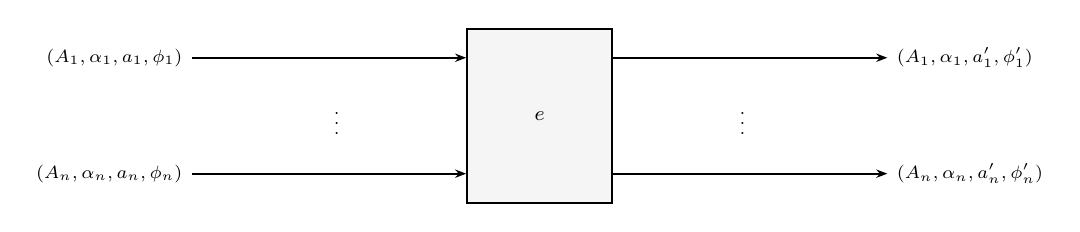
\begin{tikzpicture}[
    box/.style={draw, thick, minimum width=2cm, minimum height=2.4cm, fill=gray!8, font=\footnotesize},
    wire/.style={thick, -{Stealth[length=4pt]}},
    scale=0.92, every node/.style={scale=0.92}
  ]
  \node[box] (E) at (0,0) {$e$};

  \draw[wire] (-4.8, 0.8) node[left,font=\scriptsize]{$(A_1,\alpha_1,a_1,\phi_1)$} -- (E.west |- 0,0.8);
  \node[font=\scriptsize] at (-2.8, 0) {$\vdots$};
  \node[font=\scriptsize] at (2.8, 0) {$\vdots$};
  \draw[wire] (-4.8,-0.8) node[left,font=\scriptsize]{$(A_n,\alpha_n,a_n,\phi_n)$} -- (E.west |- 0,-0.8);

  \draw[wire] (E.east |- 0,0.8) -- (4.8, 0.8) node[right,font=\scriptsize]{$(A_1,\alpha_1,a'_1,\phi'_1)$};
  \draw[wire] (E.east |- 0,-0.8) -- (4.8,-0.8) node[right,font=\scriptsize]{$(A_n,\alpha_n,a'_n,\phi'_n)$};
\end{tikzpicture}
\end{center}

For this to be a valid event, two conditions must hold:
\begin{enumerate}[label=\textbf{(C\arabic*)}]
\item $\displaystyle\sum_i \phi'_i = \sum_i \phi_i$ \hfill (local conservation of value),
\item $(\phi_i,\phi'_i) \in T_{a_i}$ and $a'_i = f_{a_i}(\phi_i,\phi'_i)$ for all $i$ \hfill (behavioral consistency).
\end{enumerate}

\textbf{(C1)} says that within a single event, resources are redistributed, not generated.  This is a local, momentary condition---it would only amount to a global conservation law if $V$ captured all resources in the economy, which the formalism deliberately does not require.

\textbf{(C2)} says each agent acts according to its own coalgebra: the trade $(\phi_i, \phi'_i)$ must be acceptable in state $a_i$, and the new state must be the one the coalgebra dictates.

\begin{example}\label{ex:event}
Alice is in state \texttt{eager} with portfolio $\phi_A = (1000, 0)$; Bob is in state \texttt{hold} with $\phi_B = (200, 20)$.  An event in which Alice buys 3 shares from Bob at \$100 each:

\begin{center}
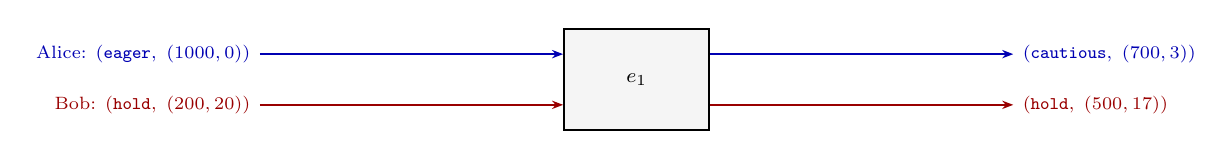
\begin{tikzpicture}[
    box/.style={draw, thick, minimum width=2cm, minimum height=1.4cm, fill=gray!8, font=\footnotesize},
    wire/.style={thick, -{Stealth[length=4pt]}},
    alicewire/.style={thick, blue!70!black, -{Stealth[length=4pt]}},
    bobwire/.style={thick, red!60!black, -{Stealth[length=4pt]}},
    scale=0.92, every node/.style={scale=0.92}
  ]
  \node[box] (E) at (0,0) {$e_1$};

  \draw[alicewire] (-5.2, 0.35) node[left,font=\scriptsize,text=blue!70!black]{Alice: $(\texttt{eager},\;(1000,0))$} -- (E.west |- 0,0.35);
  \draw[bobwire] (-5.2,-0.35) node[left,font=\scriptsize,text=red!60!black]{Bob: $(\texttt{hold},\;(200,20))$} -- (E.west |- 0,-0.35);

  \draw[alicewire] (E.east |- 0,0.35) -- (5.2, 0.35) node[right,font=\scriptsize,text=blue!70!black]{$(\texttt{cautious},\;(700,3))$};
  \draw[bobwire] (E.east |- 0,-0.35) -- (5.2,-0.35) node[right,font=\scriptsize,text=red!60!black]{$(\texttt{hold},\;(500,17))$};
\end{tikzpicture}
\end{center}

\noindent\emph{Conservation:} $(1000,0) + (200,20) = (700,3) + (500,17) = (1200, 20)$.

\noindent\emph{Behavioral consistency:}
\begin{itemize}[nosep]
\item Alice in state \texttt{eager} accepts buying up to 5 shares at $\leq\$102$.  The trade is 3 shares at \$100, so $(\phi_A, \phi'_A) \in T_{\texttt{eager}}$, and $\alpha_A$ sends her to \texttt{cautious}.
\item Bob in \texttt{hold} accepts selling up to 10 at $\geq\$100$.  The trade qualifies, and he stays in \texttt{hold}.
\end{itemize}
\end{example}

\medskip
\textbf{Composition.}
Two events can be placed in sequence---the output wires of the first feed into the input wires of the second---or in parallel, or in any combination the wiring allows.  Global conservation holds by induction: if each event individually conserves, so does any composite.

\bigskip
\noindent\fbox{\parbox{\dimexpr\textwidth-2\fboxsep-2\fboxrule}{%
\small\textbf{Categorical aside} (skip if you are not interested in the category theory machinery).

\smallskip
The color set is $W_V = \{(A, \alpha, a, \phi)\}$, and valid one-step events form a generating signature $\Sigma$.  The \emph{event prop} $\Event_V$ is the free $W_V$-colored symmetric strict monoidal category on $\Sigma$, with no imposed equations.  By Joyal--Street coherence, its morphisms are isomorphism classes of $W_V$-labeled string diagrams.

\smallskip
We take the \emph{free} prop because one-step events are not closed under sequential composition in general.  Consider two events composed sequentially, with an agent passing through both:

\begin{center}
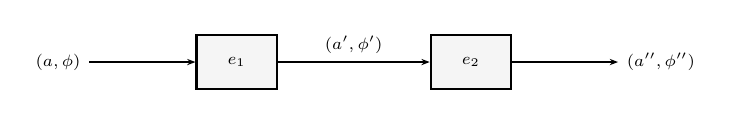
\begin{tikzpicture}[
    box/.style={draw, thick, minimum width=1.2cm, minimum height=0.8cm, fill=gray!8, font=\scriptsize},
    wire/.style={thick, -{Stealth[length=3pt]}},
    scale=0.85, every node/.style={scale=0.85}
  ]
  \node[box] (E1) at (0,0) {$e_1$};
  \node[box] (E2) at (3.5,0) {$e_2$};

  \draw[wire] (-2.2,0) node[left,font=\scriptsize]{$(a, \phi)$} -- (E1.west);
  \draw[wire] (E1.east) -- (E2.west) node[midway,above,font=\scriptsize]{$(a', \phi')$};
  \draw[wire] (E2.east) -- (5.7,0) node[right,font=\scriptsize]{$(a'', \phi'')$};
\end{tikzpicture}
\end{center}

Behavioral consistency (C2) applied to $e_1$ gives $a' = f_a(\phi, \phi')$.  Applied to $e_2$, it gives $a'' = f_{a'}(\phi', \phi'')$.  If we tried to describe the composite as a single event from $(a, \phi)$ to $(a'', \phi'')$, condition (C2) would require $a'' = f_a(\phi, \phi'')$.  But the actual value of $a''$ is
\[
f_{f_a(\phi,\phi')}(\phi', \phi''),
\]
which need not equal $f_a(\phi, \phi'')$.  Moreover, $(\phi, \phi'')$ may not even belong to $T_a$.

\smallskip
Concretely: Alice starts in \texttt{eager}; after $e_1$ she transitions to \texttt{cautious}, which has a different trade menu (buy up to 2 at $\leq\$98$ instead of up to 5 at $\leq\$102$).  A composite event from \texttt{eager} to the final state cannot be described as a single one-step event evaluated against the \texttt{eager} menu alone.

\smallskip
The free prop avoids this issue: every valid wiring of one-step events is a legitimate multi-step event, and no identifications are imposed.
}}

%% ===================================================================
\section*{Markets via the event prop}
%% ===================================================================

The event prop $\Event_V$ contains all possible trading histories consistent with conservation and behavioral consistency---every way that agents could exchange resources, in any order, with any wiring.  Most of this is far too general to describe any particular economic setting.

A \emph{market} should be some structured collection of events in $\Event_V$---the events that a particular mechanism permits.  The goal is to pick out collections corresponding to specific real-world markets, and to ask whether this framework can recover existing financial mathematics or reveal structure that was not visible before.

We begin with a common mechanism: the central limit order book.

%% ===================================================================
\section*{Limit order events}
%% ===================================================================

A central limit order book (CLOB) is a mechanism for trading financial assets---used, for example, by the New York Stock Exchange, NASDAQ, and the Chicago Mercantile Exchange.  To participate, an agent submits a \emph{limit order}: a declaration of which asset they want to buy or sell, how many units, and the most (or least) they are willing to pay per unit.  The exchange maintains a book of all standing orders.  Whenever a buy order's price meets or exceeds a sell order's price on the same asset, the two orders are matched: the trade executes at some price between the two limits, and the agents' portfolios update accordingly.

Suppose we have $n$ assets and one cash asset, so $V = \mathbb{R}^{n+1}$ with coordinates $(c, q_1, \ldots, q_n)$, where $c$ is cash and $q_k$ is the quantity of asset $k$.

\subsubsection*{Limit orders and fills}

\begin{definition}[Limit order]\label{def:limit-order}
A \emph{limit order} is a tuple $\ell = (k, s, q, p)$ where:
\begin{itemize}
\item $k \in \{1,\ldots,n\}$ is the asset,
\item $s \in \{+1,-1\}$ is the side ($+1$ = buy, $-1$ = sell),
\item $q \geq 0$ is the maximum quantity per fill ($q = 0$ means non-participation),
\item $p > 0$ is the limit price: the most a buyer will pay per unit, or the least a seller will accept.
\end{itemize}
\end{definition}

Recall that Alice, in state \texttt{eager}, was willing to buy up to 5 shares at $\leq\$102$ each.  As a limit order: $\ell_A = (1,\,+1,\,5,\,102)$.  In state \texttt{cautious}, she would submit a different order: $(1,\,+1,\,2,\,98)$.  Bob in state \texttt{hold} offers to sell up to 10 shares at $\geq\$100$: $\ell_B = (1,\,-1,\,10,\,100)$.

\begin{definition}[Fill]\label{def:fill}
A \emph{fill} of a limit order $\ell = (k, s, q, p)$ consists of an execution quantity $q' \in (0,q]$ and an execution price $p^*$ satisfying $p^* \leq p$ if $s = +1$ (buy), or $p^* \geq p$ if $s = -1$ (sell).  The fill changes the holder's portfolio by
\[
\delta(\ell,\, q',\, p^*) \;=\; (\underbrace{-s\,q'\,p^*}_{\text{cash}},\; 0, \ldots, \underbrace{s\,q'}_{\text{asset } k}, \ldots, 0).
\]
\end{definition}

The event in Example~\ref{ex:event} was a fill: Alice's order $\ell_A = (1,+1,5,102)$ was filled at $q' = 3$, $p^* = 100$, giving $\delta(\ell_A, 3, 100) = (-300, 3)$.  Bob's order filled symmetrically: $\delta(\ell_B, 3, 100) = (+300, -3)$.  The two changes sum to zero---conservation.

\subsubsection*{Limit order agents}

\begin{definition}[Portfolio limit order]
A \emph{portfolio limit order} is a tuple $L = (\ell_1, \ldots, \ell_n)$, one limit order per asset.  Non-participation in asset $k$ is indicated by setting $q_k = 0$ in $\ell_k$.
\end{definition}

\begin{definition}[Limit order agent]
A \emph{limit order agent} is a pair $w = (\phi, L)$: a portfolio $\phi \in V$ and a portfolio limit order $L$.
\end{definition}

This is the simplest model of a CLOB participant: a portfolio and a standing set of orders.  Note that this is \emph{not} rich enough to model Alice---her limit order depends on her internal state, and this definition has no state.  We will return to this point.

\subsubsection*{Fill events}

\begin{definition}[Fill event]\label{def:fill-event}
A \emph{fill event} among limit order agents $w_1 = (\phi_1, L_1), \ldots, w_m = (\phi_m, L_m)$ is a finite set of fills
\[
\mathcal{F} = \bigl\{(i_{\mathrm{buy}},\, \ell_{\mathrm{buy}},\; i_{\mathrm{sell}},\, \ell_{\mathrm{sell}},\; q',\; p^*)\bigr\}
\]
each pairing a buy order from agent $i_{\mathrm{buy}}$ with a sell order from agent $i_{\mathrm{sell}}$ on the same asset, with execution price between the two limits and quantity within both per-fill caps.  Each agent's portfolio updates by the sum of deltas from all fills they participate in.  The limit orders do not change: the same $L_i$ appear on input and output.
\end{definition}

\begin{center}
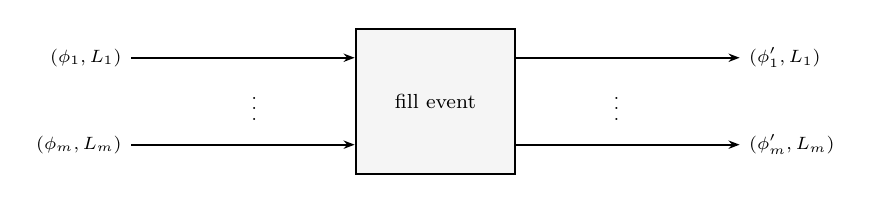
\begin{tikzpicture}[
    box/.style={draw, thick, minimum width=2.2cm, minimum height=2cm, fill=gray!8, font=\footnotesize},
    wire/.style={thick, -{Stealth[length=4pt]}},
    scale=0.92, every node/.style={scale=0.92}
  ]
  \node[box] (E) at (0,0) {fill event};

  \draw[wire] (-4.2, 0.6) node[left,font=\scriptsize]{$(\phi_1, L_1)$} -- (E.west |- 0,0.6);
  \node[font=\scriptsize] at (-2.5, 0) {$\vdots$};
  \node[font=\scriptsize] at (2.5, 0) {$\vdots$};
  \draw[wire] (-4.2,-0.6) node[left,font=\scriptsize]{$(\phi_m, L_m)$} -- (E.west |- 0,-0.6);

  \draw[wire] (E.east |- 0,0.6) -- (4.2, 0.6) node[right,font=\scriptsize]{$(\phi'_1, L_1)$};
  \draw[wire] (E.east |- 0,-0.6) -- (4.2,-0.6) node[right,font=\scriptsize]{$(\phi'_m, L_m)$};
\end{tikzpicture}
\end{center}

For instance, the event in Example~\ref{ex:event} is a fill event when Alice and Bob are viewed as limit order agents:

\begin{center}
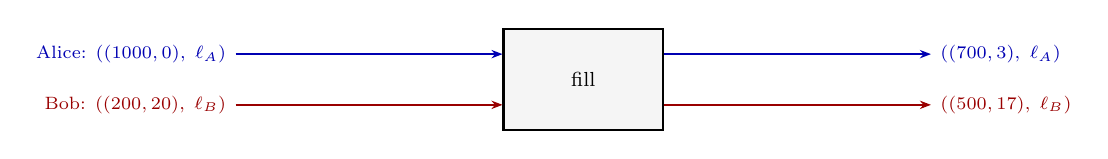
\begin{tikzpicture}[
    box/.style={draw, thick, minimum width=2.2cm, minimum height=1.4cm, fill=gray!8, font=\footnotesize},
    alicewire/.style={thick, blue!70!black, -{Stealth[length=4pt]}},
    bobwire/.style={thick, red!60!black, -{Stealth[length=4pt]}},
    scale=0.92, every node/.style={scale=0.92}
  ]
  \node[box] (E) at (0,0) {fill};

  \draw[alicewire] (-4.8, 0.35) node[left,font=\scriptsize,text=blue!70!black]{Alice: $((1000,0),\;\ell_A)$} -- (E.west |- 0,0.35);
  \draw[bobwire] (-4.8,-0.35) node[left,font=\scriptsize,text=red!60!black]{Bob: $((200,20),\;\ell_B)$} -- (E.west |- 0,-0.35);

  \draw[alicewire] (E.east |- 0,0.35) -- (4.8, 0.35) node[right,font=\scriptsize,text=blue!70!black]{$((700,3),\;\ell_A)$};
  \draw[bobwire] (E.east |- 0,-0.35) -- (4.8,-0.35) node[right,font=\scriptsize,text=red!60!black]{$((500,17),\;\ell_B)$};
\end{tikzpicture}
\end{center}

Conservation is automatic: each fill transfers $q'p^*$ cash from buyer to seller and $q'$ units of asset from seller to buyer, netting to zero across all agents.

\subsubsection*{Fill events compose}

A natural question: what happens when we wire fill events together---some agents from one fill event feeding into another, with arbitrary wiring?  For example, three agents might participate in two fill events, with one agent's output from the first feeding into the second:

\begin{center}
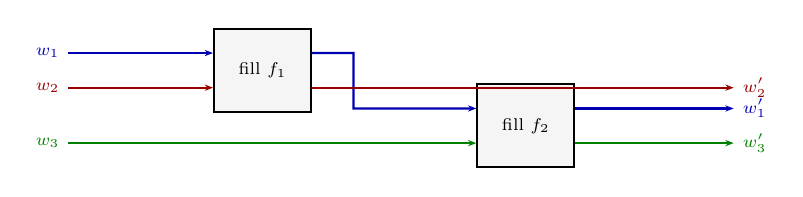
\begin{tikzpicture}[
    box/.style={draw, thick, minimum width=1.4cm, minimum height=1.2cm, fill=gray!8, font=\scriptsize},
    wire/.style={thick, -{Stealth[length=3pt]}},
    alicewire/.style={thick, blue!70!black, -{Stealth[length=3pt]}},
    bobwire/.style={thick, red!60!black, -{Stealth[length=3pt]}},
    carolwire/.style={thick, green!50!black, -{Stealth[length=3pt]}},
    scale=0.88, every node/.style={scale=0.88}
  ]
  \node[box] (E1) at (0,0.4) {fill $f_1$};
  \node[box] (E2) at (3.8,-0.4) {fill $f_2$};

  % inputs to f1
  \draw[alicewire] (-2.8, 0.65) node[left,font=\scriptsize,text=blue!70!black]{$w_1$} -- (E1.west |- 0,0.65);
  \draw[bobwire]   (-2.8, 0.15) node[left,font=\scriptsize,text=red!60!black]{$w_2$} -- (E1.west |- 0,0.15);

  % f1 output: w1' feeds into f2, w2' exits
  \draw[alicewire] (E1.east |- 0,0.65) -- ++(0.6,0) -- ++(0,-0.8) -- (E2.west |- 0,-0.15);
  \draw[bobwire]   (E1.east |- 0,0.15) -- (6.8,0.15) node[right,font=\scriptsize,text=red!60!black]{$w'_2$};

  % w3 input to f2
  \draw[carolwire] (-2.8,-0.65) node[left,font=\scriptsize,text=green!50!black]{$w_3$} -- ++(2.6,0) -- ++(0,0) -- (E2.west |- 0,-0.65);

  % f2 outputs
  \draw[alicewire] (E2.east |- 0,-0.15) -- (6.8,-0.15) node[right,font=\scriptsize,text=blue!70!black]{$w'_1$};
  \draw[carolwire] (E2.east |- 0,-0.65) -- (6.8,-0.65) node[right,font=\scriptsize,text=green!50!black]{$w'_3$};
\end{tikzpicture}
\end{center}

It turns out that any such composite is itself achievable by a single fill event.

\begin{proposition}\label{prop:fill-compose}
Let $D$ be any string diagram built by wiring fill events together (sequentially, in parallel, or any combination) in which limit order agents $w_1, \ldots, w_m$ enter with portfolios $\phi_1, \ldots, \phi_m$ and exit with portfolios $\phi'_1, \ldots, \phi'_m$, all with the same limit orders $L_i$ throughout.  Then there exists a single fill event with the same input and output.
\end{proposition}

\begin{proof}
The diagram $D$ contains some number of fill events, each consisting of a finite set of individual fills.  Let $\mathcal{F}$ be the union of all individual fills across every event in $D$.  We claim $\mathcal{F}$ is a valid set of fills for a single fill event among $w_1, \ldots, w_m$.

Each fill in $\mathcal{F}$ pairs a buy order $\ell_{\mathrm{buy}}$ from some agent $i$ with a sell order $\ell_{\mathrm{sell}}$ from some agent $j$ on the same asset, at an execution price between the two limits and a quantity within both per-fill caps.  These validity conditions depend only on the limit orders---not on the agents' current portfolios.  Since the limit orders are the same at every stage of the diagram (they never change), every fill that was valid at an intermediate stage is equally valid at the start.

The net portfolio change for each agent $i$ is the sum of the $\delta$-changes from all fills involving agent $i$.  This sum is the same whether the fills are spread across multiple events or collected into one.

Conservation: each individual fill conserves (buyer's loss equals seller's gain), so their union conserves.
\end{proof}

\medskip
The limit order setting, as defined, has no notion of multi-step complexity.  Any trading history among limit order agents---no matter how many intermediate events---is indistinguishable (in its net effect) from a single simultaneous fill.  This is not a defect of the model; it reflects a genuine feature of central limit order books.  When orders arrive at an exchange, the book matches them without regard to the sequence in which they were submitted---what matters is the set of standing orders and which ones are compatible.

But the collapse also exposes what this model \emph{cannot} do.  Alice, whose willingness to trade depends on an internal state that updates after each event, is not a limit order agent in this sense.  Her behavior is inherently multi-step: what she will accept next depends on what has already happened.  To capture agents like Alice, we need state.

%% ===================================================================
\section*{Limit order events with state}
%% ===================================================================

A \emph{stateful limit order agent} has a set of internal states, and in each state, it presents a portfolio limit order.  After participating in a fill event, it transitions to a new state---possibly changing the orders it presents next.

\begin{definition}[Stateful limit order agent]\label{def:stateful-lo}
A \emph{stateful limit order agent} is a tuple $(S, s_0, \lambda, \tau, \phi)$ where:
\begin{itemize}
\item $S$ is a finite set of states, with initial state $s_0 \in S$,
\item $\lambda\colon S \to \{\text{portfolio limit orders}\}$ assigns a portfolio limit order to each state,
\item $\tau\colon S \times \{\text{valid fills of } \lambda(s)\} \to S$ is a transition map: after a fill in state $s$, the agent moves to state $\tau(s, \text{fill})$,
\item $\phi \in V$ is the current portfolio.
\end{itemize}
\end{definition}

Alice is now modelable.  With one asset ($n = 1$), a portfolio limit order is a single limit order.  She has $S = \{\texttt{eager}, \texttt{cautious}\}$ with $s_0 = \texttt{eager}$, and:
\[
\lambda(\texttt{eager}) = \bigl((1,+1,5,102)\bigr), \qquad \lambda(\texttt{cautious}) = \bigl((1,+1,2,98)\bigr).
\]
After any fill in state \texttt{eager}, she transitions to \texttt{cautious}.  In \texttt{cautious}, she stays.

A \emph{stateful fill event} is defined just as before---a set of matched fills among participating agents---but now the output wires carry updated states as well as updated portfolios.  Each agent's fill must be valid against the limit order presented in their \emph{current} state, and the output state is determined by the transition rule.

Does the composition property still hold?  Not in general.  After a fill, an agent may transition to a state with different limit orders.  A fill that was valid against the old orders may not be valid against the new ones.  This is exactly the situation we encountered with the event prop: Alice in \texttt{eager} accepts trades that Alice in \texttt{cautious} does not.  A multi-step history through intermediate state changes cannot, in general, be collapsed to a single step.

This begins to look like the event prop itself.  A stateful limit order agent is an $F_V$-coalgebra whose trade menus are restricted to limit-order-shaped trades: in each state, the set of acceptable portfolio swaps is exactly the set of fills of the limit order presented in that state.  The transition map sends each fill to the successor state.  Fill events satisfying conservation and behavioral consistency are generators of a prop---and because one-step events no longer compose, the right object is the free prop on these generators.

\begin{remark}[The progression]
Without state, limit order events compose trivially---everything collapses to a single step.  With state, they do not---and the resulting structure mirrors the event prop, restricted to agents whose preferences take the shape of limit orders.
\end{remark}

%% ===================================================================
\section*{Avenues for Investigation}
%% ===================================================================

\begin{question}
The functor $F_V(A) = \coprod_{T \subseteq V \times V} A^T$ does not appear to carry comonad structure: a counit $\varepsilon\colon F_V \to \mathrm{Id}$ would require extracting an element of $A$ from a pair $(T, f\colon T \to A)$, but $T$ may be empty.  What changes if we require every trade menu to be nonempty (the null trade is always available)?  Would $F_V$ then be a comonad, and would the coalgebra condition be meaningful?
\end{question}

\begin{question}
Condition (C1) is a local, instantaneous conservation law.  It would only amount to a global conservation law if $V$ captured all resources in the economy.  What happens when multiple event props, over different portfolio spaces, interact?  Is there a meaningful notion of ``open system'' in which local conservation holds but global conservation can fail?
\end{question}

\begin{question}
As noted in the categorical aside above, one-step events in $\Event_V$ are closed under sequential composition if and only if the coalgebra satisfies
\[
f_{f_a(\phi_1,\phi_2)}(\phi_2,\phi_3) \;=\; f_a(\phi_1,\phi_3)
\]
for all composable pairs $(\phi_1,\phi_2) \in T_a$ and $(\phi_2,\phi_3) \in T_{f_a(\phi_1,\phi_2)}$.  Characterize the $F_V$-coalgebras satisfying this condition.  Does it coincide with a known categorical notion?
\end{question}

\begin{question}
What natural quotients of $\Event_V$ are economically meaningful?  Identifying morphisms with the same endpoints gives a preorder; is there an intermediate quotient that retains some causal structure?
\end{question}

\begin{question}
A stateful limit order agent determines an $F_V$-coalgebra with limit-order-shaped trade menus.  Is there a useful functor in the reverse direction---from general $F_V$-coalgebras to stateful limit order agents?  A coalgebraic agent may exhibit cyclic trade preferences (willing to trade $A \to B$, $B \to C$, $C \to A$) that no limit order can represent, suggesting no such functor exists in general.
\end{question}

%% ===================================================================
\section*{References}
%% ===================================================================
\begin{itemize}[leftmargin=*]
\item A.\ Joyal, R.\ Street, \emph{The geometry of tensor calculus~I}, Adv.\ Math.\ \textbf{88} (1991), 55--112.
\item P.\ Selinger, \emph{A survey of graphical languages for monoidal categories}, Lect.\ Notes Phys.\ \textbf{813} (2011), 289--355.
\end{itemize}

\end{document}
